% GENERATED by make_paper_assets.py -- do not edit by hand.
\begin{figure}[t]
\centering
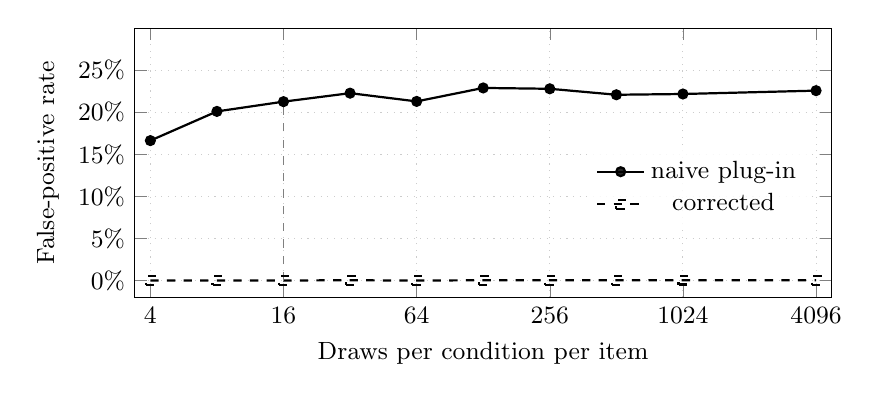
\begin{tikzpicture}
\begin{semilogxaxis}[
  width=0.86\columnwidth, height=5.0cm, log basis x=2,
  xlabel={Draws per condition per item}, ylabel={False-positive rate},
  xmin=3.4, xmax=4800, ymin=-0.02, ymax=0.30,
  ytick={0,0.05,0.1,0.15,0.2,0.25}, yticklabels={0\%,5\%,10\%,15\%,20\%,25\%},
  xtick={4,16,64,256,1024,4096}, xticklabels={4,16,64,256,1024,4096},
  legend style={at={(0.97,0.55)}, anchor=north east, font=\small, draw=none,
                fill=white, fill opacity=0.85, text opacity=1},
  grid=major, grid style={dotted, gray!40},
  tick label style={font=\small}, label style={font=\small},
]
\addplot[thick, mark=*, mark size=1.6pt] coordinates {(4,0.1664) (8,0.2011) (16,0.2127) (32,0.2228) (64,0.2130) (128,0.2290) (256,0.2280) (512,0.2209) (1024,0.2218) (4096,0.2258)};
\addlegendentry{naive plug-in}
\addplot[thick, dashed, mark=square, mark size=1.6pt] coordinates {(4,0.0000) (8,0.0000) (16,0.0001) (32,0.0004) (64,0.0000) (128,0.0004) (256,0.0003) (512,0.0003) (1024,0.0005) (4096,0.0003)};
\addlegendentry{corrected}
\draw[gray, dashed] (axis cs:16,-0.02) -- (axis cs:16,0.2127);
\end{semilogxaxis}
\end{tikzpicture}
\caption{False-positive rate of the compatibility certificate versus sampling
budget, under a null resampled from the real full-panel disclosure rates and
answer-law skew (8{,}000 replications per point, full grid in
Table~\ref{tab:calibration}). The dashed vertical marks the 16-draw budget used
throughout. The naive certificate does not approach zero with more data: it
plateaus at 21--23\% out to 4{,}096 draws, 256$\times$ our budget,
because near-total disclosure leaves no slack to absorb sampling noise. The
per-item corrected certificate (plotted) stays at or below 0.05\% (95\% upper bounds at most
0.13\%). The family-wise regime, used for the certified violations of Section~\ref{sec:models},
rejected none of the 8{,}000 replications at any draw count (Table~\ref{tab:calibration}).}
\label{fig:calibration}
\end{figure}
